\documentclass[12pt]{article}
\usepackage[utf8]{inputenc}
\usepackage[brazil]{babel}
\usepackage[margin = 1in]{geometry}
\usepackage{graphicx}
\usepackage{subfigure}
\usepackage{minted}
\usepackage{indentfirst}
\usepackage{float}
\usepackage{multirow}
\usepackage{textcomp}


\begin{document}

    
\begin{titlepage}
 \vfill
  \begin{center}
   {\large \textbf{UNIVERSIDADE FEDERAL DO PARANÁ \\ SETOR DE TECNOLOGIA \\ DEPARTAMENTO DE ENGENHARIA ELÉTRICA}} \\[5cm]

  {\large {Marco Antonio Rios  GRR20133243 \\ Wendeurick Silverio GRR20134722} }\\[4cm]


   {\Large \textbf{Projetos de Sistemas Digitais em PLD - TE087} \\ Laboratório 8}\\[6cm]
    \vfill

    \vspace{2cm}

    \large \textbf{Curitiba}

    \large \textbf{\today}

      \end{center}
\end{titlepage}

\clearpage
%\tableofcontents    
%\clearpage
%-------------------------------------------------------------
\section{Desafio 1}
O primeiro desafio propõe a implementação de uma máquina de estados capaz de reconhecer sequencias de quatro ou mais 0's ou 1's consecutivos.
\subsection{Implementação}
A máquina de estados finitos foi projetada em 2 ramos, além do estado inicial: sequencia de zeros (estados 0A, 0B, 0C e 0D) e sequencia de uns (estados 1A, 1B, 1C e 1D), totalizando 9 estados.

O circuito foi projetado para transitar nas bordas de subida do \emph{clock} e, ao detectar uma sequencia de quatro ou mais 0's ou 1's, a saída permanece em nível alto, caso contrário, em nível baixo.

Abaixo, o diagrama de transição de estados, onde \emph{in} representa a entrada, \emph{out} a saída e \emph{rst} o \emph{reset}. 

\begin{figure}[!h]
    \centering
    \includegraphics[width=1.0\textwidth]{lab8_sequence_detector.png}
    \caption{Diagrama da máquina de estados.}
\end{figure}

A estimativa da quantidade de \emph{flip-flops} tipo D (DFF) para esta máquina de estados é:
\begin{itemize}  
\item Codificação sequencial (binária): \begin{math}log_{2}(9)\approx 3,17\end{math} : 4 DFF
\item Codificação "one-hot": um por estado: 9 DFF
\end{itemize}

Abaixo, o código \emph{VHDL} da implementação.

\inputminted{vhdl}{sequence_detector.vhd}

Abaixo, os sumários de utilização de dispositivos para as codificações sequencial e \emph{one-hot}. Nota-se que a quantidade de DFF (aqui, \emph{Number of Slice Flip Flops}) está de acordo com a estimativa.

\begin{figure}[!h]
    \centering
    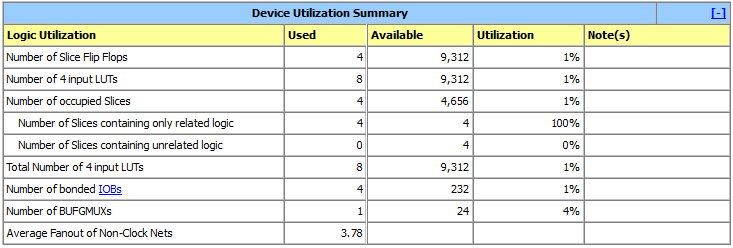
\includegraphics[width=1.0\textwidth]{lab8_sequence_detector_dff_seq.png}
    \caption{Sumário da codificação sequencial.}
\end{figure}

\begin{figure}[!h]
    \centering
    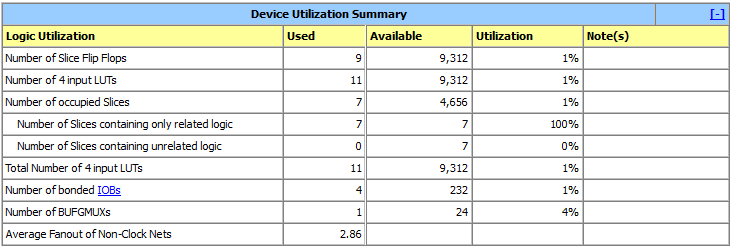
\includegraphics[width=1.0\textwidth]{lab8_sequence_detector_dff_onehot.png}
    \caption{Sumário da codificação \emph{one-hot}.}
\end{figure}

\subsection{Simulação}

Abaixo, o código \emph{VHDL} do \emph{Testbench}.

\inputminted{vhdl}{sequencer_detector_tb.vhd}



Abaixo, o diagrama temporal do Testbench.

\begin{figure}[!h]
    \centering
    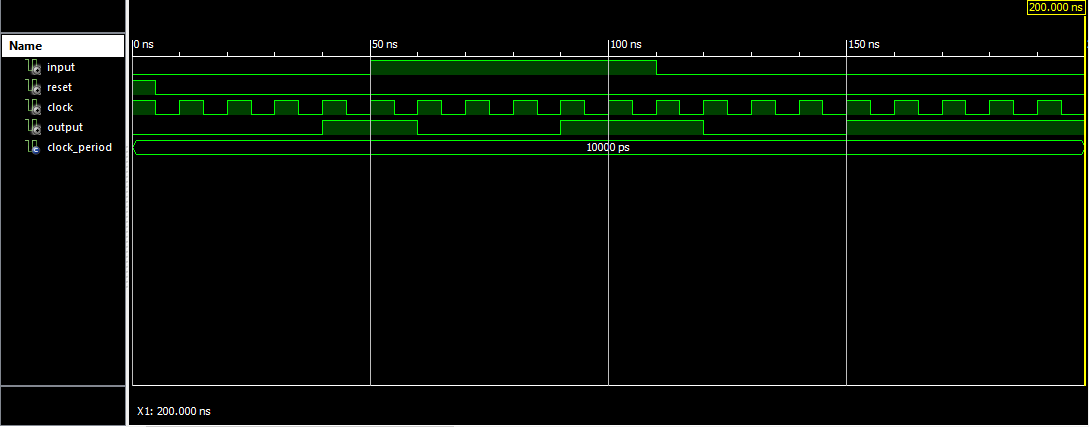
\includegraphics[width=1.0\textwidth]{lab8_sequence_detector_tb.png}
    \caption{Testbench do desafio1.}
\end{figure}

A simulação está de acordo com o proposto. Ao detectar 4 entradas iguais consecutivas, a partir da 5ª borda de subida do clock, a saída permanece em nível alto enquanto não houver mudança na entrada. Caso haja tal mudança, a saída retorna ao nível baixo na próxima borda de subida.


\clearpage
%-------------------------------------------------------------
\section{Desafio 2}
O desafio 2 consiste em criar um gerador de sinal, composto apenas por um sinal de clock como entrada e um sinal de saída. A regra para compor a onda de saída é que por 20 períodos de clock o sinal fique em nível lógico alto e após isso, por 40 períodos em nível lógico baixo. A máquina de estado teoricamente teria 60 estados, mas para simplificação, é possível adicionar um contador e facilitar na programação. Adicionando o contador, a nossa máquina de estado terá somente dois estados, como visto na figura \ref{fsm2}. Para haver mudança do estado HIGH para o estado LOW, é necessário que o tempo t seja igual a um período de T1, que no caso é 20 periodos de clock, e que esteja em uma borda de subida, x ='1'. Da mesma forma, uma mudança do estado LOW para o estado HIGH só ocorre quando o tempo t é igual a T2, que no caso é 40.

\begin{figure}[!h]
    \centering
    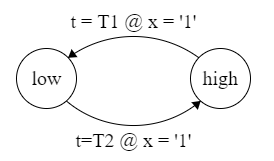
\includegraphics[width=0.4\textwidth]{fsm2.PNG}
    \caption{Maquina de estados do desafio2.}
    \label{fsm2}
\end{figure}

O número de estados necessários para a implementação desse circuito, segue a regra descrita no item anterior, então as estimativas ficariam: 

\begin{itemize}  
\item Codificação sequencial (binária): \begin{math}log_{2}(60)\approx 5.8\end{math} : 6 DFF
\item Codificação "one-hot": um por estado: 60 DFF
\end{itemize}


\subsection{Implementação}

\inputminted{vhdl}{desafio2.vhd}

\subsection{Simulação}

Abaixo, o código \emph{VHDL} do Testbench.

\inputminted{vhdl}{desafio2_tb.vhd}

\begin{figure}[!h]
    \centering
    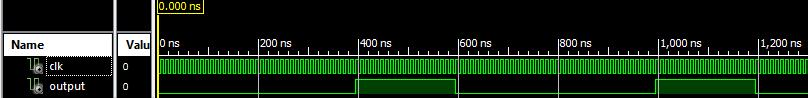
\includegraphics[width=1.0\textwidth]{desafio2_tb.png}
    \caption{Testbench do desafio2.}
\end{figure}



Apos a implementação, constatou-se que o número de DFF ficou próximo do número previsto quando a codificação foi sequencial, no caso, 7 DFFs, e quando o esquema de codificação foi alterado, pode-se observar uma diferença nos resultados esperados, os DFFs continuaram os mesmos 7. Talvez o programa não permita o uso excessivo de DFFs para essa função.



\begin{figure}[!h]
    \centering
    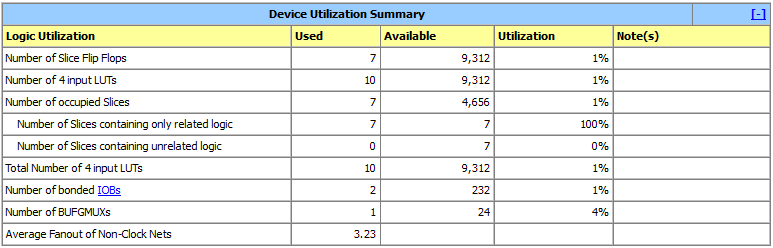
\includegraphics[width=1.0\textwidth]{jesus.PNG}
    \caption{Sumário da codificação sequencial.}
\end{figure}


\clearpage
%-------------------------------------------------------------
\section{Desafio 3}
O desafio 3 consiste em um contador de 0 a F. A maquina de estados tem 16 estados. Para fins visuais, ela deve completar um ciclo em 1 segundo. 

A estimativa de DFFs deve ser feita antes de considerar o tempo. A estimativa seria de:

\begin{itemize}  
\item Codificação sequencial (binária): \begin{math}log_{2}(16)\approx 4\end{math} : 4 DFF
\item Codificação "one-hot": um por estado: 16 DFF
\end{itemize}

Esta estimativa é atendida neste caso, como visto nas figuras:

\begin{figure}[!h]
    \centering
    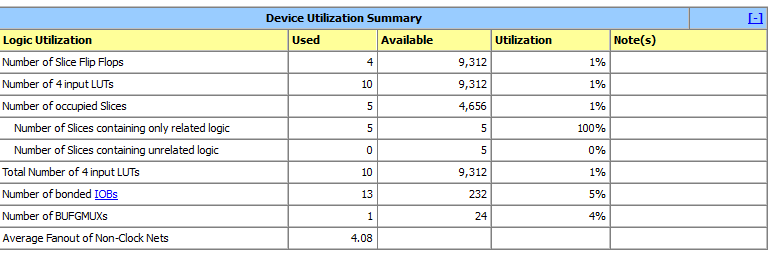
\includegraphics[width=1.0\textwidth]{agora2.PNG}
    \caption{Sumário da codificação sequencial.}
\end{figure}

\begin{figure}[!h]
    \centering
    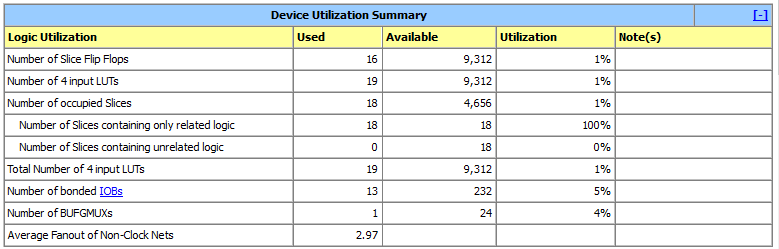
\includegraphics[width=1.0\textwidth]{agora.PNG}
    \caption{Sumário da codificação \emph{one-hot}.}
\end{figure}

\begin{figure}[!h]
    \centering
    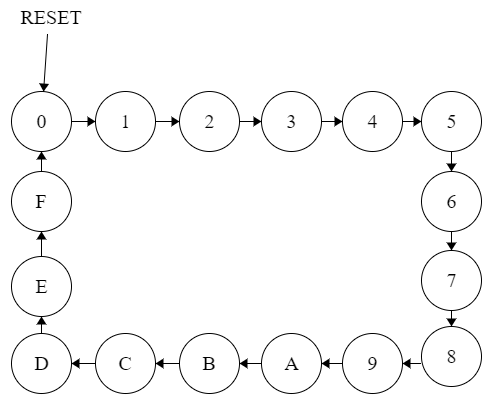
\includegraphics[width=1.0\textwidth]{fsm3.png}
    \caption{Máquina de estados do desafio3}
\end{figure}

\subsection{Implementação}

Abaixo, o código \emph{VHDL} da implementação do componente display de 7 segmentos.

\inputminted{vhdl}{display7seg.vhd}

Abaixo, o código \emph{VHDL} da implementação do contador.

\inputminted{vhdl}{desafio3.vhd}

\subsection{Mapeamento das portas I/0}

Abaixo, o mapeamento das entradas e saídas para o kit Nexys2.

\inputminted{vhdl}{desafio3_pins.ucf}

\subsection{Simulação}

Abaixo, o código \emph{VHDL} do Testbench.

\inputminted{vhdl}{des3_tb.vhd}

\begin{figure}[!h]
    \centering
    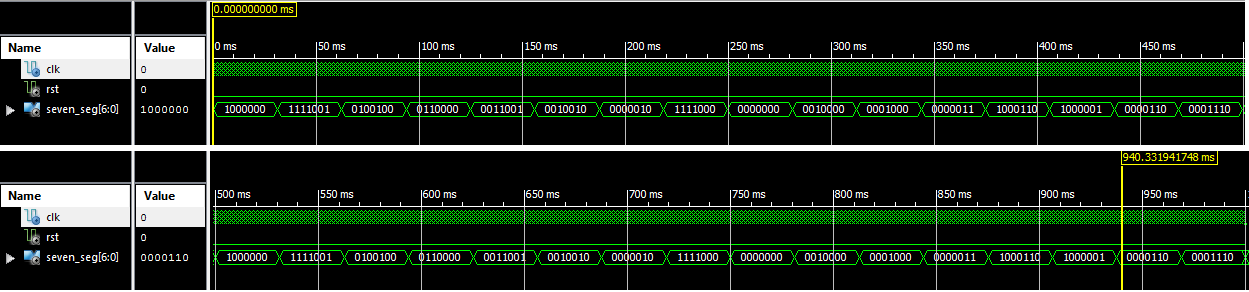
\includegraphics[width=1.0\textwidth]{desafio3_tb.png}
    \caption{Testbench do desafio3.}
\end{figure}

\end{document}
